%%%%%%%%%%%%%%%%%%%%%%%%%%%%%%%%%%%%%%%%%%%%%%%%%%%%%%%%%%%%%%%%%%%%%%%%%%%%%%%%%%%%%%%%%
\begin{frame}
  \frametitle{A choice of terminology}
  % logistic regression
  \begin{block}{Logistic regression (binary classification)}
    \begin{columns}
      %%%%%%%%%%%%%%%%%%%%%%%%%%%%%%%%% 
      % dot product + function 
      \begin{column}{0.4\textwidth}
        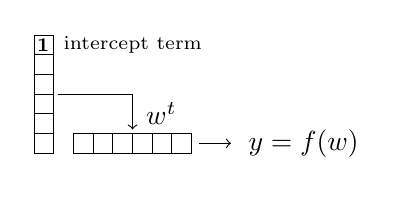
\begin{tikzpicture}
          \only<1->{
            % x
            \draw[step=.25] (0,-0) grid (0.25, 1.5);%
            \node (x) at (0.05,-0.25) {$\x$};%
            \node (bias) at (0.115,1.37) {\scriptsize{\textbf{1}}};
            \node[anchor=west] (bias2) at (0.25,1.37) {\scriptsize{intercept term}};
            
            % w^t
            \draw[step=.25] (0.49,0) grid (2.0, 0.25);%
            \node[anchor=west] (w) at (1.3,0.5) {$\seq{w^t}$};%
            \draw (0.3,0.75) -- (1.25,0.75);%
            \draw[->] (1.25,0.75) -- (1.25,0.3);%
            % res 1
            \draw[->] (2.1,0.125) -- (2.5,0.125);%
            \node[anchor=west] (y) at (2.6,0.125) {$y =
              f( \scal{ \seq{w}}{\x})$};%
          }
        \end{tikzpicture}
        $$ 
        f(a=\scal{\seq{w}}{\x}) = \frac{e^{a}}{1+e^{a}} = \sigma(a)
        $$
      \end{column}
      % the logistic regression
      \begin{column}{0.6\textwidth}
        \begin{center}
          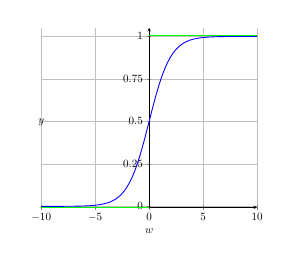
\begin{tikzpicture}[scale=0.4]
            \begin{axis}%
              [ %%%%%%%%%%%%%%%%%
              grid=major, %
              xmin=-10, % 
              xmax=10, % 
              axis x line=bottom, % 
              ytick={0,.25,.5,.75,1.0}, %
              ymax=1.05, % 
              axis y line=middle, % 
              xlabel = $\scal{\seq{w}}{\x}$, %
              ylabel = $y$, % 
              every  axis y label/.style={at={(current axis.north  west)},above=2mm} ]% 
              %%%%%%%%% binary classif in green
              \addplot%
              [ blue,thick,%
              mark=none, samples=100, domain=-10:10, ]
              (x,{1/(1+exp(-x))});
              \addplot%
              [ green,very thick,%
              mark=none, samples=100, domain=0:10, ]
              (x,{1.005});
              \addplot%
              [ green,very thick,%
              mark=none, samples=100, domain=-10:0, ]
              (x,{-0.005});
            \end{axis}
          \end{tikzpicture}
        \end{center}
      \end{column}
    \end{columns}
  \end{block}
  %%%%%%%% neuronal view 
  \pause
  \begin{block}{A single artificial neuron}
    \begin{columns}
      %%%%%%%%%%%%%%%%%%% left 
      \begin{column}{0.4\textwidth}
        \begin{tikzpicture}
          % neurone 1
          \draw[red] (1,1) circle (0.1cm);% output 1
          \node[anchor=west] (ny1) at (1.5,1){{\color{red}{ $y=f( \scal{\seq{w}}{\x})$}}};
          % input
          \node (nx) at (-0.75,0.625){$\x$}; %
          \draw[snake=brace] (-0.45,-0.125) -- (-0.45,1.375); 
          \node (bias) at (-0.25,1.25){\scriptsize{\textbf{1}}}; %
          \node[anchor=west] (bias2) at (-0.25,1.5){\scriptsize{bias term}}; %
          % draw neurons
          \node[color=red] (nw) at (0.55,0.1){$\seq{w}$}; %
          \foreach \y in {0,0.25,...,1.25}{ \draw (0,\y) circle (0.1cm);%
            \draw[->-,red] (0.125,\y) -- (0.875,1); }
          \draw[fill=black] (0,1.25) circle (0.1cm);% bias neuron
        \end{tikzpicture}
      \end{column}
      %%%%%%%%%%%%%%%%%%% right
      \begin{column}{0.6\textwidth}
        \begin{itemize}
        \item pre-activation : $a= \scal{\seq{w}}{\x}$
        \item $f$: activation function 
        \item Input values =  input ``neurones''
        \item $\x$: a vector of values, a layer
        \end{itemize}
      \end{column}
    \end{columns}
  \end{block}
\end{frame}



%%%%%%%%%%%%%%%%%%%%%%%%%%%%%%%%%%%%%%%%%%%%%%%%% 
\begin{frame}{A choice of terminology - 2}
  \begin{block}{From binary classification to $\nclasses$ classes (Maxent)}
    \begin{columns}
      %%%%%%%%%%%%%%%%%%%%%%%%%%%%%%%%% 
      % dot product + function 
      \begin{column}{0.5\textwidth}
        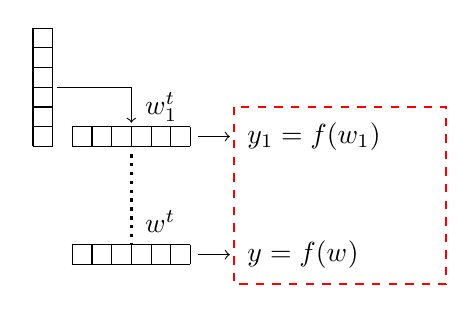
\begin{tikzpicture}
          {
            % x
            \draw[step=.25] (0,-0) grid (0.25, 1.5);%
            \node (x) at (0.05,-0.25) {$\x$};%
            
            % w^t
            \draw[step=.25] (0.49,0) grid (2.0, 0.25);%
            \node[anchor=west] (w) at (1.3,0.5) {$\seq{w_1^t}$};%
            \draw (0.3,0.75) -- (1.25,0.75);%
            \draw[->] (1.25,0.75) -- (1.25,0.3);%
            % res 1
            \draw[->] (2.1,0.125) -- (2.5,0.125);%
            \node[anchor=west] (y) at (2.6,0.125) {$y_1 =
              f( \scal{ \seq{w_1}}{\x})$};%
          }
          {
            % res k
            \draw[dotted, very thick] (1.25,-0.1) -- (1.25,-1.25);%
            \begin{scope}[yshift=-1.5cm]
              \draw[step=.25] (0.49,0) grid (2.0, 0.25);%
              \node[anchor=west] (wk) at (1.3,0.5) {$\seq{w_{\nclasses}^t}$};%
              \draw[->] (2.1,0.125) -- (2.5,0.125);%
              \node[anchor=west] (y) at (2.6,0.125) {$y_{\nclasses} =
                f(\scal{\seq{w_{\nclasses}}}{\x})$};%
            \end{scope}
          }
          {% square together the output
            \draw[red,dashed,thick] (2.55, 0.5) rectangle (5.25,-1.75);
          }
        \end{tikzpicture}
      \end{column}
      % the maxent function
      \begin{column}{0.5\textwidth}
        \begin{align*}
          y_k &= f(a_k=\scal{\seq{w_k}}{\x})= P(c=k|\x)\\
              &= \frac{e^{a_k}}{\color{red}\sum_{k'=1}^{\nclasses} e^{a_{k'}}}= \frac{e^{a_k}}{\color{red}Z(\x)} \\
          \sum_{k=1}^{\nclasses} y_k &= \sum_{k=1}^{\nclasses}P(c=k|\x) =1 
        \end{align*}
      \end{column}
    \end{columns}
  \end{block}
  %%%%%%%% neuronal view 
  \pause
  \begin{block}{A simple neural network}
    \begin{columns}
      \begin{column}{0.5\textwidth}
        \begin{tikzpicture}
          % neurone 1
          \draw[red] (1,1) circle (0.1cm);% output 1
          \node[anchor=west,red] (ny1) at (1.5,1){$y_1=
            f(\seq{w_1^t}\x)$}; %
          % input
          \node (nx) at (-0.5,0.625){$\x$}; %
          \node[color=red] (nw) at (0.5,1.4){$\seq{w_1}$}; %
          \foreach \y in {0,0.25,...,1.25}{ \draw (0,\y) circle
            (0.1cm);%
            \draw[->-,red] (0.125,\y) -- (0.875,1); }
          
          \draw[snake=brace] (-0.2,-0.125) -- (-0.2,1.375);

          % neurone {\nclasses}
          
          \foreach \a in {0.75}{ \draw[green] (1,1-\a) circle
            (0.1cm);% output 2
            \node[color=green] (nw2) at (0.5,-0.25){ $\seq{w_{\nclasses}}$}; %
            \node[anchor=west,green] (ny2) at (1.5,1-\a){$y_{\nclasses}=
              f(\seq{w_{\nclasses}^t}\x)$}; %

            \foreach \y in {0,0.25,...,1.25}{ \draw[->-,green]
              (0.125,\y) -- (0.875,1-\a); }
            % dotted between output neurones:
            \draw[dotted,very thick] (1,0.9) -- (1,0.35);

          }
        \end{tikzpicture}
        % 
      \end{column}
      \begin{column}{0.5\textwidth}
        \begin{itemize}
        \item $\x$: \emph{input layer}
        \item $\seq{y}$: \emph{output layer}
        \item each $y_k$ has its parameters $\seq{w}_k$
        \item $f$ is the \important{softmax} function
        \end{itemize}
      \end{column}
    \end{columns}
  \end{block}
\end{frame}

%%%%%%%%%%%%%%%%%%%%%%%%%%%%%%%%%%%%%%%%%%%%%%%%%%%%%%%%%%%%%%%%%%%%%%%%%%%%%%% 
%%%%%%%% use the cancel package 
\begin{frame}{Refresher: Matrix and Vector product}
  \begin{center}
    \begin{tabular}{rllr}
      $ \vct{y}$ &\ $=\ \W$ &$\ \times\ \x$ \\[2ex]
      %%%%%%%% line with figs 
      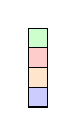
\begin{tikzpicture}

        \draw[fill=green!20] (0,0.5) rectangle (0.25, 0.25);
        \draw[fill=red!20] (0,0.25) rectangle (0.25, 0.0);
        \draw[fill=orange!20] (0,0.0) rectangle (0.25, -0.25);
        \draw[fill=blue!20] (0,-0.25) rectangle (0.25, -0.5);
        \draw[step=.25] (0,-0.5) grid (0.25, 0.5);
      \end{tikzpicture}
      
                &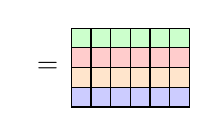
\begin{tikzpicture}
                          \node at (-0.3,-0) {$=$};
        \draw[fill=green!20] (0,0.5) rectangle (1.5, 0.25);
        \draw[fill=red!20] (0,0.25) rectangle (1.5, 0.0);
        \draw[fill=orange!20] (0,0.0) rectangle (1.5, -0.25);
        \draw[fill=blue!20] (0,-0.25) rectangle (1.5, -0.5);
        \draw[step=.25] (0,-0.5) grid (1.5, 0.5);
      \end{tikzpicture}

      &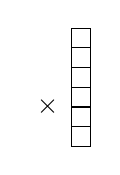
\begin{tikzpicture}
        \node at (-0.3,-0.25) {$\times$};
        \draw[step=.25] (0,-0.75) grid (0.25, 0.75);
      \end{tikzpicture}\\[2ex]
      %%%%%
      \color{green!60}$y_1$ &\color{green}$\ =\ \W_{1,:}$ &$\  \times\ \x$\\
      \color{red!60}$y_2$ &\color{red!60}$\ =\ \W_{2,:}$ &$\  \times\ \x$\\
      \ $\cdots$ &\ $\cdots$ &$\ \cdots$
    \end{tabular}
\end{center}
In terms of dimension: 
\begin{displaymath}
  \textrm{With } \left\{
    \begin{array}{ll}
      \x  &: (L_1 \times 1)\\
      \W  &: (L_2 \times C_2)\\
      \seq{y} &: (L_2 \times 1)
    \end{array} \right. \Rightarrow (\W\x) :
   (L_2 \times 1)= (L_2 \times \underbrace{\xcancel{C_2) (L_1 } }_{\color{red}C_2=L_1} \times 1)
\end{displaymath}
\end{frame}

%%%%%%%%%%%%%%%%%%%%%%%%%%%%%%%%%%%%%%%%%%%%%%%%%%%%%%%%%%%%%%%%%%%%%%%%%%%%%%% 
%%%%%%%% use the cancel package 
\begin{frame}{Refresher: Matrix-matrix product}
  $\seq{X}$ is a matrix of 2 columns, 2 vectors as $\x$: 
  \begin{center}
    \begin{tabular}{rllr}
      $ \seq{Y}$ &\ $=\W$ &$\ \times\ \seq{X}$ \\[2ex]
      %%%%%%%% line with figs 
      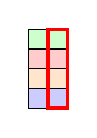
\begin{tikzpicture}
        % matrix Y 
        \draw[fill=green!20] (0,0.5) rectangle (0.5, 0.25);
        \draw[fill=red!20] (0,0.25) rectangle (0.5, 0.0);
        \draw[fill=orange!20] (0,0.0) rectangle (0.5, -0.25);
        \draw[fill=blue!20] (0,-0.25) rectangle (0.5, -0.5);
        \draw[step=.25] (0,-0.5) grid (0.5, 0.5);
        \draw[draw=red,very thick] (0.25,-0.5) rectangle (0.5, 0.5);
      \end{tikzpicture}
      % matrix W
                &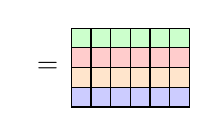
\begin{tikzpicture}
                          \node at (-0.3,-0) {$=$};
        \draw[fill=green!20] (0,0.5) rectangle (1.5, 0.25);
        \draw[fill=red!20] (0,0.25) rectangle (1.5, 0.0);
        \draw[fill=orange!20] (0,0.0) rectangle (1.5, -0.25);
        \draw[fill=blue!20] (0,-0.25) rectangle (1.5, -0.5);
        \draw[step=.25] (0,-0.5) grid (1.5, 0.5);
      \end{tikzpicture}
      % Matrix X 
      &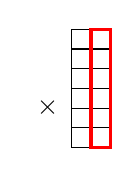
\begin{tikzpicture}
        \node at (-0.3,-0.25) {$\times$};
        \draw[step=.25] (0,-0.75) grid (0.5, 0.75);
        \draw[draw=red,very thick] (0.25,-0.75) rectangle (0.5, 0.75);
      \end{tikzpicture}
      %%%%%
    \end{tabular}
\end{center}
In terms of dimension: 
\begin{displaymath}
  \textrm{With } \left\{
    \begin{array}{ll}
      \seq{X}  &: (L_1 \times C_1)\\
      \W  &: (L_2 \times C_2)\\
      \seq{y} &: (L_2 \times C_1)
    \end{array} \right. \rightarrow
   (L_2 \times C_2)= (L_2 \times \underbrace{\xcancel{C_2) (L_1 } }_{\color{red}C_2=L_1} \times C_1)
\end{displaymath}
\end{frame}



%%%%%%%%%%%%%%%%%%%%%%%%%%%%%%%%%%%%%%%%%%%%%%%%%%%%%%%%%%%%%%%%%%%%%%%%%%%%%%% 
\begin{frame}
  \frametitle{Two layers fully connected}
  \begin{center}
    \begin{tikzpicture}
      \begin{scope}
        % input
        \node (nx) at (-0.7,0.625){$\x$}; %
        \foreach \y in {0,0.25,...,1.25}{ 
          \draw (0,\y) circle  (0.1cm);%
        }
        \draw (-0.2,-0.2) rectangle (0.2,1.5);
        \draw[snake=brace] (-0.4,-0.125) -- (-0.4,1.375); 
        % output
        \foreach \y in {0.25,0.5,...,1}{ 
          \draw (1.5,\y) circle  (0.1cm);%
        }
        \draw (1.3,0.05) rectangle (1.7,1.2);
        \draw (0.2,-0.2) -- (1.3,0.05); 
        \draw (0.2,1.5) -- (1.3,1.2);
        \draw[dotted, thick] (0.2,1.5) -- (1.3,0.05);
        \draw[dotted,thick] (0.2,-0.2) -- (1.3,1.2); 
        \draw[snake=brace] ( 1.8, 1.2) --(1.8, 0.05) ; 
        \node[anchor=west] (ny) at (1.9,0.625){$\seq{y}=f(\W \x)$}; %
        \node[anchor=west] (nW) at (0.83,-0.75){$\W$};%
        \node[anchor=west] (nW) at (0.83,-1.25) {$\W_{k,:}=\seq{w_k}^t$}; %
        \draw[->]  (0.83,-0.7) -- (0.83,0.6);%
      \end{scope}
      %%%%%%%%%%%%%%%%%%%%%%%%%%%%%%%%%%%%%%%%%% 
      %% matrix view 
      %%%%%%%%%%%%%%%%%%%%%%%%%%%%%%%%%%%%%%%%%% 
      \only<2->{
        \begin{scope}[xshift=6cm,yshift=0.15cm]
          
          \draw[->] (-1.75,0.5) -- (-0.7,0.5);
          \draw[step=.25] (0,-0) grid (1.5, 1);%
          \draw[step=.25] (1.99,-0.25) grid (2.25, 1.25 );%
          \draw[step=.25] (2.99,-0) grid (3.25, 1 );%
          % oper
          \node[anchor=west] (times) at (1.4, 0.5) {$\times$};
          \node[anchor=west] (equals) at (2.4, 0.5) {$=$};
          % names
          \node[anchor=west] (f) at (-0.6, 0.5) {$f\Big($};
          \node[anchor=west] (fe) at (2.2, 0.5) {$\Big)$};
          \node[anchor=west] (W) at (0.25, -0.5) {$\seq{W}$};
          \node[anchor=west] (x) at (1.75, -0.5) {$\seq{x}$};
          \node[anchor=west] (x) at (3, -0.5) {$\seq{y}$};
        \end{scope}
      }
    \end{tikzpicture}
  \end{center}
  \pause\pause
  {
    \begin{columns}
      \column{0.5\textwidth}
      Activation $f$:
      \begin{itemize}
      \item $f$ is usually a non-linear function
      \item $f$ is a component wise function
      \item tanh, sigmoid, relu, ...
      \end{itemize}
      \column{0.5\textwidth}
      Dimensions: 
      \begin{itemize}
      \item $\x: \nfeats \times 1 $
      \item $\seq{W}: \nclasses \times \nfeats $
      \item $\seq{y}: (\nclasses \times \xcancel{ \nfeats) \times (  \nfeats }
        \times 1 ) =\nclasses \times 1 $
      \end{itemize}
    \end{columns}
    \textit{e.g} the softmax function:
    $$      
    y_k = P(c=k|\x) = \frac{e^{\scal{\seq{w_k}}{\x}} }{\sum_{k'}e^{\scal{\seq{w_{k'}}}{\x}}}
    = \frac{e^{\W_{k,:}\x}}{\sum_{k'} e^{\W_{k',:}\x}}
    $$   
  }
\end{frame}





%%%%%%%%%%%%%%%%%%%%%%%%%%%%%%%%%%%%%%%%%%%%%%%%%%%%%%%%%%%%%%%%%%%%%%%%%%%%%%% 
\begin{frame}{Bias or not bias}
  \begin{block}{Implicit Bias}
    \begin{center}
      \begin{tikzpicture}
        \begin{scope}
          % input

        \node (nx) at (-0.9,0.625){$\x$}; %
        \draw[snake=brace] (-0.6,-0.125) -- (-0.6,1.375); 

        \foreach \y in {0,0.25,...,1.25}{ 
          \draw (0,\y) circle  (0.1cm);%
        }
        \draw (-0.2,-0.2) rectangle (0.2,1.5);        
        % the first node is a constant set to one 
        \draw[fill=red] (0,1.25) circle  (0.1cm);%
        \node[red] (nx) at (-0.4,1.25){$1$}; %
        
        

        % output
        \foreach \y in {0.25,0.5,...,1}{ 
          \draw (1.5,\y) circle  (0.1cm);%
        }
        \draw (1.3,0.05) rectangle (1.7,1.2);
        \draw (0.2,-0.2) -- (1.3,0.05); 
        \draw (0.2,1.5) -- (1.3,1.2);
        \draw[dotted, thick] (0.2,1.5) -- (1.3,0.05);
        \draw[dotted,thick] (0.2,-0.2) -- (1.3,1.2); 
        \draw[snake=brace] ( 1.8, 1.2) --(1.8, 0.05) ; 
        \node[anchor=west] (ny) at (1.9,0.625){$\seq{y}=f(\W \x)$}; %
        \node[anchor=west] (nW) at (0.83,-0.75){$\W$};%
        \node[anchor=west] (nW) at (0.83,-1.25) {$\W_{k,:}=\seq{w_k}^t$}; %
        \draw[->]  (0.83,-0.7) -- (0.83,0.6);%
      \end{scope}
      %%%%%%%%%%%%%%%%%%%%%%%%%%%%%%%%%%%%%%%%%% 
      %% matrix view 
      %%%%%%%%%%%%%%%%%%%%%%%%%%%%%%%%%%%%%%%%%% 
        \begin{scope}[xshift=6cm,yshift=0.15cm]

          % bias term in x 
          \draw[fill=red] (1.99,1) rectangle (2.25, 1.25 );%
          % bias term in W 
          \draw[fill=red] (0,-0) rectangle (0.25, 1);%
          % grids for matrix and vectors
          \draw[->] (-1.75,0.5) -- (-0.7,0.5);
          \draw[step=.25] (0,-0) grid (1.5, 1);%
          \draw[step=.25] (1.99,-0.25) grid (2.25, 1.25 );%
          \draw[step=.25] (2.99,-0) grid (3.25, 1 );%
          % oper
          \node[anchor=west] (times) at (1.4, 0.5) {$\times$};
          \node[anchor=west] (equals) at (2.4, 0.5) {$=$};
          % names
          \node[anchor=west] (f) at (-0.6, 0.5) {$f\Big($};
          \node[anchor=west] (fe) at (2.2, 0.5) {$\Big)$};
          \node[anchor=west] (W) at (0.25, -0.5) {$\seq{W}$};
          \node[anchor=west] (x) at (1.75, -0.5) {$\seq{x}$};
          \node[anchor=west] (x) at (3, -0.5) {$\seq{y}$};
        \end{scope}
    \end{tikzpicture}
  \end{center}
  \end{block}

  \begin{block}{Explicit bias}
    \begin{center}
      \begin{tikzpicture}
        \begin{scope}
          % input

        \node (nx) at (-0.9,0.625){$\x$}; %
        \draw[snake=brace] (-0.6,-0.125) -- (-0.6,1.125); 

        \foreach \y in {0,0.25,...,1}{ 
          \draw (0,\y) circle  (0.1cm);%
        }
        \draw (-0.2,-0.2) rectangle (0.2,1.25);        

        % output
        \foreach \y in {0.25,0.5,...,1}{ 
          \draw (1.5,\y-0.125) circle  (0.1cm);%
        }
        \draw (1.3,0.05-0.125) rectangle (1.7,1.2-0.125);
        \draw (0.2,-0.2) -- (1.3,0.05-0.125); 
        \draw (0.2,1.25) -- (1.3,1.2-0.125);
        \draw[dotted, thick] (0.2,1.25) -- (1.3,0.05-0.125);
        \draw[dotted,thick] (0.2,-0.2) -- (1.3,1.2-0.125); 
        \draw[snake=brace] ( 1.8, 1.2-0.125) --(1.8, 0.05-0.125) ; 
        \node[anchor=west] (ny) at (1.9,0.625){$\seq{y}=f(\W \x + \seq{b})$}; %
      \end{scope}
      %%%%%%%%%%%%%%%%%%%%%%%%%%%%%%%%%%%%%%%%%% 
      %% matrix view 
      %%%%%%%%%%%%%%%%%%%%%%%%%%%%%%%%%%%%%%%%%% 
        \begin{scope}[xshift=6cm,yshift=0.15cm]
          \draw[->] (-1.25,0.5) -- (-0.7,0.5);

          \draw[fill=red] (2.99,-0) rectangle (3.25, 1 );% bias in red
          % grids for matrix and vectors
          \draw[step=.25] (0,-0) grid (1.5, 1);% W 
          \draw[step=.25] (1.99,-0.25) grid (2.25, 1.25 );% x
          \draw[step=.25] (2.99,-0) grid (3.25, 1 );% b
          \draw[step=.25] (3.99,-0) grid (4.25, 1 );% y 
          % oper
          \node[anchor=west] (times) at (1.4, 0.5) {$\times$};
          \node[anchor=west] (equals) at (2.4, 0.5) {$+$};
          \node[anchor=west] (equals) at (3.4, 0.5) {$=$};
          % names
          \node[anchor=west] (f) at (-0.6, 0.5) {$f\Big($};
          \node[anchor=west] (fe) at (3.2, 0.5) {$\Big)$};
          \node[anchor=west] (W) at (0.25, -0.5) {$\seq{W}$};
          \node[anchor=west] (x) at (1.75, -0.5) {$\seq{x}$};
          \node[anchor=west] (x) at (3, -0.5) {$\seq{b}$};
          \node[anchor=west] (x) at (4, -0.5) {$\seq{y}$};
        \end{scope}
    \end{tikzpicture}
  \end{center}

  \end{block}
\end{frame}


%%%%%%%%%%%%%%%%%%%%%%%%%%%%%%%%%%%%%%%%%%%%%%%%%%%%%%%%%%%%%%%%%%%%%%%%
\begin{frame}{Classification with a simple neural network}
  \begin{block}{Binary classification}
    \begin{itemize}
    \item The input layer is a vector ($\x$), it encodes the data
    \item A single output neuron transform $\x$,  $\seq{w}$ are its parameters
    \item With a sigmoïd activation, the loss function is the binary cross entropy, the log-loss,
      minus the log-likelihood, ...
    \end{itemize}
  \end{block}
  \begin{block}{Multiclass}
    \begin{itemize}
    \item The input layer is a vector ($\x$) 
    \item The output layer $\y$ contains one neuron per class  
    \item It transforms $\x$, $\W$ are the parameters of the output layer
    \item $\W$ gathers the $\seq{w}_k= \W_{k,:}$
    \item With a softmax activation, the loss function is the cross entropy, the log-loss,
      minus the log-likelihood, ...
    \end{itemize}
  \end{block}
  \begin{center}
    {\color{red} Other loss functions exist for classification}
  \end{center}
\end{frame}

%%%%%%%%%%%%%%%%%%%%%%%%%%%%%%%%%%%%%%%%%%%%%%%%%%%%%%%%%%%%%%%%%%%%%%%%
\begin{frame}{Regression with a simple neural network}
  \begin{block}{Simple linear regression}
    $$
    y = f_{\params} (\x),\  y\in\real
    $$
    \begin{itemize}
    \item The input layer is a vector ($\x$), it encodes the data
    \item A single output neuron for $y$ ($\seq{w}$ are its parameters)
    \item The activation function depends on the output domain
    \end{itemize}
  \end{block}
  \begin{block}{Multi-variate linear regression}
    $$
    \y = f_{\params} (\x),\  \y\in\real^{\nclasses}
    $$
    \begin{itemize}
    \item The input layer is a vector ($\x$) 
    \item The output layer $\y$ contains one neuron per output value
    \item It transforms $\x$ in $\y$, $\W$ are the parameters of the output layer
    \end{itemize}
  \end{block}
\end{frame}


%%%%%%%%%%%%%%%%%%%%%%%%%%%%%%%%%%%%%%%%%%%%%%%%%%%%%%%%%%%%%%%%%%%%%%%%
\begin{frame}{Loss for regression}
  \framesubtitle{The Mean Squarred Error \textit{a.k.a} MSE}
  \begin{align*}
\dataset &= (\exi, \y\sid{i})_{i=1}^{\nsamples}, \\
\fullloss &= \frac{1}{\nsamples} \sum_{i=1}^{\nsamples} ||\y\sid{i} - f_{\params}(\exi) ||^2
  \end{align*}
  \begin{center}
    \includegraphics[width=0.6\textwidth]{./figs/mse}
  \end{center}
  \begin{center}
    {\color{red} Other loss functions exist for regression}
  \end{center}

\end{frame}

%%%%%%%%%%%%%%%%%%%%%%%%%%%%%%%%%%%%%%%%%%%%%%%%%%%%%%%%%%%%%%%%%%%%%%%%
\begin{frame}
  \frametitle{Two layers fully connected: another view}
  \begin{center}
    \begin{tikzpicture}[scale=0.75]
      \begin{scope}
        % input
        \node (nx) at (-0.7,0.625){$\x$}; %
        \foreach \y in {0,0.25,...,1.25}{ 
          \draw (0,\y) circle  (0.1cm);%
        }
        \draw (-0.2,-0.2) rectangle (0.2,1.5);
        \draw[snake=brace] (-0.4,-0.125) -- (-0.4,1.375); 
        % output
        \foreach \y in {0.25,0.5,...,1}{ 
          \draw (1.5,\y) circle  (0.1cm);%
        }
        \draw (1.3,0.05) rectangle (1.7,1.2);
        \draw (0.2,-0.2) -- (1.3,0.05); 
        \draw (0.2,1.5) -- (1.3,1.2);
        \draw[dotted, thick] (0.2,1.5) -- (1.3,0.05);
        \draw[dotted,thick] (0.2,-0.2) -- (1.3,1.2); 
        \draw[snake=brace] ( 1.8, 1.2) --(1.8, 0.05) ; 
        \node[anchor=west] (ny) at (1.9,0.625){$\seq{y}=f(\W \x)$}; %
        \node[anchor=west] (nW) at (0.83,-0.75){$\W$};%
        \draw[->]  (0.83,-0.7) -- (0.83,0.6);%
      \end{scope}
      %%%%%%%%%%%%%%%%%%%%%%%%%%%%%%%%%%%%%%%%%% 
      %% matrix view 
      %%%%%%%%%%%%%%%%%%%%%%%%%%%%%%%%%%%%%%%%%% 
        \begin{scope}[xshift=6cm,yshift=0.15cm]
          
          \draw[<->] (-1.25,0.5) -- (-0.7,0.5);
          \draw[step=.25] (0,-0) grid (1.5, 1);%
          \draw[step=.25] (1.99,-0.25) grid (2.25, 1.25 );%
          \draw[step=.25] (2.99,-0) grid (3.25, 1 );%
          % oper
          \node[anchor=west] (times) at (1.4, 0.5) {$\times$};
          \node[anchor=west] (equals) at (2.4, 0.5) {$=$};
          % names
          \node[anchor=west] (f) at (-0.75, 0.5) {$f\Big($};
          \node[anchor=west] (fe) at (2.2, 0.5) {$\Big)$};
          \node[anchor=west] (W) at (0.25, -0.5) {$\seq{W}$};
          \node[anchor=west] (x) at (1.75, -0.5) {$\seq{x}$};
          \node[anchor=west] (x) at (3, -0.5) {$\seq{y}$};
        \end{scope}
     
    \end{tikzpicture}
  \end{center}
  This basic brick implements a transformation of $\x$ in $\seq{y} =f(\W \x)$:
  \begin{itemize}
  \item A linear transformation $\W \x$
  \item Followed by a non-linear function
  \end{itemize}
  Example: a candidate made 6 interviews $\rightarrow \x \in
  \real^{6}$
  \begin{itemize}
  \item First compute 4 new scores : $\W \x \in  \real^{4}$, each is a
    linear combination of $\x$
  \item Apply a non-linearity to get $\seq{y}$
  \end{itemize}
  \begin{center}
    
            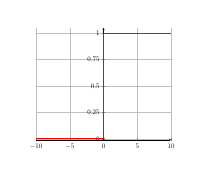
\begin{tikzpicture}[scale=0.25]
            \begin{axis}%
              [ %%%%%%%%%%%%%%%%%
              grid=major, %
              xmin=-10, % 
              xmax=10, % 
              axis x line=bottom, % 
              ytick={0,.25,.5,.75,1.0}, %
              ymax=1.05, % 
              ymin = -0.01, %
              axis y line=middle, % 
              every  axis y label/.style={at={(current axis.north
                  west)},above=2mm} ]% 
              \addplot%
              [ red,line width=0.5mm,%
              mark=none, samples=100, domain=0:10, ]
              (x,{1.00});
              \addplot%
              [ red,line width=0.5mm,%
              mark=none, samples=100, domain=-10:0, ]
              (x,{0.0});
              \addplot%
              [ red,line width=0.5mm,%
              mark=none, samples=100, domain=-10:0]
              (x,{0.0});
              \addplot[ red,line width=0.5mm,%
              mark=none] coordinates {(0,0) (0,1)};%
            \end{axis}
          \end{tikzpicture}\hfill
%%%%%%% logistic
          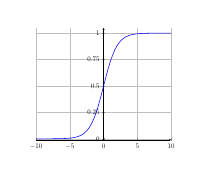
\begin{tikzpicture}[scale=0.25]
            \begin{axis}%
              [ %%%%%%%%%%%%%%%%%
              grid=major, %
              xmin=-10, % 
              xmax=10, % 
              axis x line=bottom, % 
              ytick={0,.25,.5,.75,1.0}, %
              ymax=1.05, % 
              ymin = -0.01, %
              axis y line=middle, % 
              every  axis y label/.style={at={(current axis.north
                  west)},above=2mm} ]% 
              \addplot%
              [ blue,thick,%
              mark=none, samples=100, domain=-10:10, ]
              (x,{1/(1+exp(-x))});
            \end{axis}
          \end{tikzpicture}\hfill
%%%%%%%%% relu
         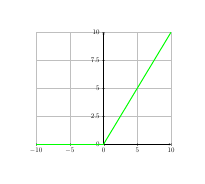
\begin{tikzpicture}[scale=0.25]
            \begin{axis}%
              [ %%%%%%%%%%%%%%%%%
              grid=major, %
              xmin=-10, % 
              xmax=10, % 
              axis x line=bottom, % 
              ytick={0,2.5,5,7.5,10}, %
              ymax=10, % 
              ymin = -0.01, %
              axis y line=middle, % 
              every  axis y label/.style={at={(current axis.north
                  west)},above=2mm} ]% 
              \addplot%
              [ green,line width=0.5mm,%
              mark=none, samples=100, domain=0:-10, ]
              (x,{0.00});
              \addplot%
              [ green,line width=0.5mm,%
              mark=none, samples=100, domain=0:10, ]
              (x,x);
            \end{axis}
          \end{tikzpicture}
  \end{center}
\end{frame}



